
% Differential treatment of Interests received from different interfaces can be achieved in a more elegant way, without reverting to probabilistic methods.

Essentially, the probabilistic Interest accept algorithm divides the available forwarding tokens between interfaces proportionally to their satisfaction ratios.
Exactly the same effect can be achieved without using probabilistic methods, simply by enabling and enforcing additional Interest limits for each incoming interface, where the values of the limits directly depend on the interface satisfaction ratios.
Additionally, routers may need to explicitly announce these limits to their downstream neighbors, ensuring that any forwarded Interest from the downstream is actually getting through, resulting in genuine Interest satisfaction statistics.

The formal definition of the dynamic limits algorithm is presented in Pseudocode~\ref{alg:dynamic limits}, while Fig.~\ref{fig:dynamic limits example} illustrates how the algorithm would work in our toy example on Fig.~\ref{fig:flooding example}.
Assuming the initial (physical) limit $L=10$ and the current satisfaction ratios on the the router A are 50\% for \texttt{eth1} and 0\% for \texttt{eth0}, and on the router B the ratio is 30\%  \texttt{eth0}, each node would set and announce the following  incoming interface limits $L'$: 
\begin{enumerate}
\item the router B would set and announce the incoming interface limit $L'=3$;
\item the router A, after receiving announcement from B would readjust its incoming interface limits to $L'_{eth1} = 1.5$ and $L'_{eth0} = 0$; and
\item legitimate user and adversary may either obey or ignore the announced limit, which will be in any case enforced by the router A.
\end{enumerate}


\begin{figure}[htbp]
  \centering
  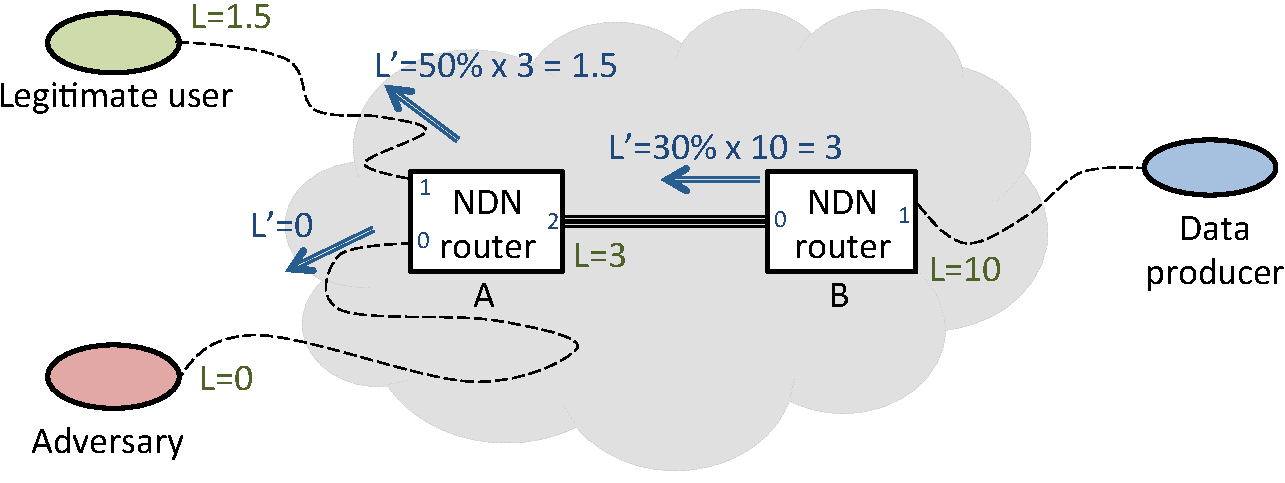
\includegraphics[scale=0.3]{dynamic-limits}
  \caption{Dynamic limits example: routers explicitly tell neighbors how many Interest can be for sure delivered to the Data producer}
  \label{fig:dynamic limits example}
\end{figure}


\floatname{algorithm}{Pseudocode}

%%%%%%%%%%%%%%%%%%%%%%%%%%%%%%
%%%%%%%%%%%%%%%%%%%%%%%%%%%%%%
%%%%%%%%%%%%%%%%%%%%%%%%%%%%%%

\begin{algorithm}[h]
\caption{Dynamic limits}
\label{alg:dynamic limits}
\begin{algorithmic}[1]
\State{} \Comment{Same initialization, InData and Timeout functions as in Physical Limits algorithm}
\vspace{0.2cm}
\State{$\forall f \in \mathrm{interfaces} : L'_{f} \leftarrow L_{f}$} \Comment{Per-incoming interface Interest limit} 

\vspace{0.2cm}

\State{} \Comment{\textit{Announcement from the neighbor}}
\Function{InLimits}{InInterface $if$, Limit $L'$}
    \State $L_{if} \leftarrow L'$
\EndFunction

\vspace{0.2cm}

\Function{AnnounceLimits}{} \Comment{\textit{E.g., every second}}
\For{\textbf{each} outgoing interface $of$}

   \For{\textbf{each} incoming interface $if$}
        \State $L'_{if}= {L_{of}} \times (1 - U_{if}/F_{if})$
        \State AnnounceLimit($if$, $L'_{if}$)
   \EndFor

\EndFor
\EndFunction

\end{algorithmic}
\end{algorithm}

The zero limit for the adversary's link means that the router A is temporarily not willing to accept any interests from this link, not until the statistics decays to the appropriate level (recall Fig.~\ref{fig:ratio example}).
At the next iterations of the dynamic limits algorithm, the legitimate user will be able to gradually improve the statistics on both the router A and router B (all his Interests will get through and will return Data), eventually resulting in a full allowance ($L'=L=10$) in the links between the routers A and B, and the user and the router A.

It should be noted that while in the description of the dynamic limits algorithm we used notions of ``outgoing'' and ``incoming'' interfaces, in the real system all interfaces can be both incoming and outgoing.
Thus, it may not be entirely clear which outgoing limit $L_{of}$ (line 10 in the algorithm) should be used to calculate the incoming limit $L_{if}$.
To overcome this problem, in our actual implementation we enforced separate incoming/outgoing interface limits for each individual FIB entry.
That is, for each FIB entry we set a separate Interest limit for each incoming interface ($L_{if}^{'FIB}$) based on a sum of FIB entry limits for each outgoing interface $L=\sum{L_{of}^{FIB}}$.


% Alex: not sure if this paragraph belongs here
Essentially, both probabilistic Interest accept and the dynamic limits algorithm are forms of a well-known push-back mechanism~\cite{Pushback}, with several core differences.
First, we are suppressing (pushing back) unwanted requests for Data, not the actual Data.
Second, differentiating between good and bad Interests is based on the traffic symmetry property of NDN.
% Alex: I'm not entirely sure about this point... 
Finally, both intelligent attack mitigation algorithms can be enabled all the time, without degrading network performance when there are no active attack.


%%% Local Variables: 
%%% mode: latex
%%% TeX-master: "../paper"
%%% End: 
